% Exemple de graphe de flot
\begin{frame}{Exemple de graphe de flot}
    \begin{tikzpicture}
        \node[node_base] (s) at (0,0) {$s$};
        \node[node_base] (r1) at (2,2) {$r_1$};
        \node[node_base] (r2) at (2,-2) {$r_2$};
        \node[node_base] (r3) at (5,2) {$r_3$};
        \node[node_base] (r4) at (5,-2) {$r_4$};
        \node[node_base] (t) at (7,0) {$t$};

        \path[directed_edge] (s) edge node[above,sloped] {\textcolor{blue}{11}/16} (r1);
        \path[directed_edge] (s) edge node[below,sloped] {\textcolor{blue}{8}/13} (r2);
        \path[directed_edge] (r1) edge node[above,sloped] {\textcolor{blue}{12}/12} (r3);
        \path[directed_edge] (r2) edge node[below,sloped] {\textcolor{blue}{1}/4} (r1);
        \path[directed_edge] (r2) edge node[below,sloped] (capa) {\textcolor{blue}{11}/14} (r4);
        \path[directed_edge] (r3) edge node[below,sloped] {\textcolor{blue}{4}/9} (r2);
        \path[directed_edge] (r3) edge node[above,sloped] {\textcolor{blue}{15}/20} (t);
        \path[directed_edge] (r4) edge node[below,sloped] {\textcolor{blue}{7}/7} (r3);
        \path[directed_edge] (r4) edge node[below,sloped] {\textcolor{blue}{4}/4} (t);

        \node[below left=1.5cm and 0.4cm of s,align=center] (slabel) {noeud\\source};
        \node[below right=1.5cm and 0.4cm of t,align=center] (tlabel) {noeud\\terminal};
        \draw[->,thick,red] (slabel) -- (s);
        \draw[->,thick,red] (tlabel) -- (t);

        \node[below =of capa] (capalabel) {\textcolor{blue}{flot} / capacité};
        \node[ellipse,draw,red,thick,minimum width=12mm,minimum height=8mm,inner sep=0pt] (circlecapa) at (capa.center) {};
        \draw[->, thick, red] (capalabel) -- (circlecapa);
    \end{tikzpicture}
\end{frame}

\begin{frame}{Propriétés du flot}
    Un flot $f$ réalisable doit vérifier les propriétés suivantes :

    \begin{block}{Règle flot-capacité}
        Le flot d'une arête ne peut pas dépasser sa capacité.
        \[
        \forall\, u,v\in V^2\quad 0 \leq f(u,v)\leq c(u,v)
        \]
    \end{block}

    \begin{block}{Règle de conservation du flot}
        À l'exception de $s$ et $t$, le flot entrant dans un n\oe{}ud est égal au flot en sortant.
        \[
            \forall\, u\in V\setminus\{s,t\}\quad\sum_{v\in V}f(u,v) = \sum_{v\in V} f(v,u)
        \]
    \end{block}
\end{frame}

\begin{frame}{Propriétés du flot}
    \begin{block}{Flot total}
        Le flot sortant de $s$ est égal à celui entrant dans $t$.
        \[
            \sum_{u\in V}f(s,u) = \sum_{u\in V}f(u,t)
        \]
    \end{block}

    \begin{block}{Valeur du flot}
        La valeur du flot $f$, notée $\varphi$ est donnée par :
        \[
            \varphi = \sum_{u\in V}f(s,u) = \sum_{u\in V}f(u,t)
        \]
    \end{block}

    Le problème du flot maximal consiste à trouver un flot $f$ ayant la valeur du flot maximale $\varphi_{max}$
\end{frame}

\begin{frame}{Algorithme de Ford-Fulkerson}
    \begin{block}{Ford-Fulkerson}
        L'algorithme de Ford-Fulkerson est un algorithme glouton qui permet de calculer le flot maximal dans un graphe de flot.
        \medskip

        Complexité : $O((|V|+|E|)\times \varphi_{max})$
    \end{block}

    \textbf{Remarque 1} : l'algorithme de Ford-Fulkerson n'impose aucune contrainte sur le type de parcours à effectuer. En pratique, on fait un DFS.
    \medskip

    \textbf{Remarque 2} : une variante de l'algorithme qui s'appuie sur le BFS (l'algorithme d'Edmonds-Karp) permet d'obtenir une complexité en $O(|V|\times|E|^2)$, indépendante de $\varphi_{max}$.
\end{frame}

\begin{frame}{Algorithme de Ford-Fulkerson}
    \begin{center}
        \tikzstyle{edge} = [draw,thick,-]
        \tikzstyle{selected edge} = [draw,line width=3pt,-,dodgerblue!50]
        \begin{tikzpicture}[scale=0.65,every node/.style={scale=0.8},baseline]

        \node at (3.5,3.5) {\em Graphe de flot};

        \node[node_base] (s) at (0,0) {$s$};
        \node[node_base] (r1) at (2,2) {$r_1$};
        \node[node_base] (r2) at (2,-2) {$r_2$};
        \node[node_base] (r3) at (5,2) {$r_3$};
        \node[node_base] (r4) at (5,-2) {$r_4$};
        \node[node_base] (t) at (7,0) {$t$};

        \path<beamer:1-3>[edge,->] (s)  -- node[above,sloped] {\textcolor{blue}{0}/16} (r1);
        \path<beamer:1-3>[edge,->] (s)  -- node[below,sloped] {\textcolor{blue}{0}/13} (r2);
        \path<beamer:1-3>[edge,->] (r1) -- node[above,sloped] {\textcolor{blue}{0}/12} (r3);
        \path<beamer:1-3>[edge,->] (r2) -- node[below,sloped] {\textcolor{blue}{0}/4} (r1);
        \path<beamer:1-3>[edge,->] (r2) -- node[below,sloped] {\textcolor{blue}{0}/14} (r4);
        \path<beamer:1-3>[edge,->] (r3) -- node[below,sloped] {\textcolor{blue}{0}/9} (r2);
        \path<beamer:1-3>[edge,->] (r3) -- node[above,sloped] {\textcolor{blue}{0}/20} (t);
        \path<beamer:1-3>[edge,->] (r4) -- node[below,sloped] {\textcolor{blue}{0}/4} (t);
        \path<beamer:1-3>[edge,->] (r4) -- node[below,sloped] {\textcolor{blue}{0}/7} (r3);

        \path<beamer:4-6>[edge,->] (s)  -- node[above,sloped] {\textcolor{blue}{4}/16} (r1);
        \path<beamer:4-6>[edge,->] (s)  -- node[below,sloped] {\textcolor{blue}{0}/13} (r2);
        \path<beamer:4-6>[edge,->] (r1) -- node[above,sloped] {\textcolor{blue}{4}/12} (r3);
        \path<beamer:4-6>[edge,->] (r2) -- node[below,sloped] {\textcolor{blue}{0}/4} (r1);
        \path<beamer:4-6>[edge,->] (r2) -- node[below,sloped] {\textcolor{blue}{4}/14} (r4);
        \path<beamer:4-6>[edge,->] (r3) -- node[below,sloped] {\textcolor{blue}{4}/9} (r2);
        \path<beamer:4-6>[edge,->] (r3) -- node[above,sloped] {\textcolor{blue}{0}/20} (t);
        \path<beamer:4-6>[edge,->] (r4) -- node[below,sloped] {\textcolor{blue}{4}/4} (t);
        \path<beamer:4-6>[edge,->] (r4) -- node[below,sloped] {\textcolor{blue}{0}/7} (r3);

        \path<beamer:7-9>[edge,->] (s)  -- node[above,sloped] {\textcolor{blue}{12}/16} (r1);
        \path<beamer:7-9>[edge,->] (s)  -- node[below,sloped] {\textcolor{blue}{0}/13} (r2);
        \path<beamer:7-9>[edge,->] (r1) -- node[above,sloped] {\textcolor{blue}{12}/12} (r3);
        \path<beamer:7-9>[edge,->] (r2) -- node[below,sloped] {\textcolor{blue}{0}/4} (r1);
        \path<beamer:7-9>[edge,->] (r2) -- node[below,sloped] {\textcolor{blue}{4}/14} (r4);
        \path<beamer:7-9>[edge,->] (r3) -- node[below,sloped] {\textcolor{blue}{4}/9} (r2);
        \path<beamer:7-9>[edge,->] (r3) -- node[above,sloped] {\textcolor{blue}{8}/20} (t);
        \path<beamer:7-9>[edge,->] (r4) -- node[below,sloped] {\textcolor{blue}{4}/4} (t);
        \path<beamer:7-9>[edge,->] (r4) -- node[below,sloped] {\textcolor{blue}{0}/7} (r3);

        \path<beamer:10-12>[edge,->] (s)  -- node[above,sloped] {\textcolor{blue}{12}/16} (r1);
        \path<beamer:10-12>[edge,->] (s)  -- node[below,sloped] {\textcolor{blue}{4}/13} (r2);
        \path<beamer:10-12>[edge,->] (r1) -- node[above,sloped] {\textcolor{blue}{12}/12} (r3);
        \path<beamer:10-12>[edge,->] (r2) -- node[below,sloped] {\textcolor{blue}{0}/4} (r1);
        \path<beamer:10-12>[edge,->] (r2) -- node[below,sloped] {\textcolor{blue}{4}/14} (r4);
        \path<beamer:10-12>[edge,->] (r3) -- node[below,sloped] {\textcolor{blue}{0}/9} (r2);
        \path<beamer:10-12>[edge,->] (r3) -- node[above,sloped] {\textcolor{blue}{12}/20} (t);
        \path<beamer:10-12>[edge,->] (r4) -- node[below,sloped] {\textcolor{blue}{4}/4} (t);
        \path<beamer:10-12>[edge,->] (r4) -- node[below,sloped] {\textcolor{blue}{0}/7} (r3);

        \path<beamer:13-15>[edge,->] (s)  -- node[above,sloped] {\textcolor{blue}{12}/16} (r1);
        \path<beamer:13-15>[edge,->] (s)  -- node[below,sloped] {\textcolor{blue}{11}/13} (r2);
        \path<beamer:13-15>[edge,->] (r1) -- node[above,sloped] {\textcolor{blue}{12}/12} (r3);
        \path<beamer:13-15>[edge,->] (r2) -- node[below,sloped] {\textcolor{blue}{0}/4} (r1);
        \path<beamer:13-15>[edge,->] (r2) -- node[below,sloped] {\textcolor{blue}{11}/14} (r4);
        \path<beamer:13-15>[edge,->] (r3) -- node[below,sloped] {\textcolor{blue}{0}/9} (r2);
        \path<beamer:13-15>[edge,->] (r3) -- node[above,sloped] {\textcolor{blue}{19}/20} (t);
        \path<beamer:13-15>[edge,->] (r4) -- node[below,sloped] {\textcolor{blue}{4}/4} (t);
        \path<beamer:13-15>[edge,->] (r4) -- node[below,sloped] {\textcolor{blue}{7}/7} (r3);

        \end{tikzpicture}
        \hfill
        \begin{tikzpicture}[scale=0.65,every node/.style={scale=0.8},baseline]

        \node at (3.5,3.5) {\em Graphe résiduel};

        \node[node_base] (s) at (0,0) {$s$};
        \node[node_base] (r1) at (2,2) {$r_1$};
        \node[node_base] (r2) at (2,-2) {$r_2$};
        \node[node_base] (r3) at (5,2) {$r_3$};
        \node[node_base] (r4) at (5,-2) {$r_4$};
        \node[node_base] (t) at (7,0) {$t$};

        \path<beamer:2>[edge,->] (s) -- node[above,sloped] {\textcolor{forestgreen}{16}} (r1);
        \path<beamer:3-4>[selected edge,->] (s) -- node[above,sloped] {\textcolor{forestgreen}{16}} (r1);
        \path<beamer:2-3>[edge,->] (s) -- node[below,sloped] {\textcolor{forestgreen}{13}} (r2);
        \path<beamer:2>[edge,->] (r1) -- node[above,sloped] {\textcolor{forestgreen}{12}} (r3);
        \path<beamer:3-4>[selected edge,->] (r1) -- node[above,sloped] {\textcolor{forestgreen}{12}} (r3);
        \path<beamer:2-3>[edge,->] (r2) -- node[below,sloped] {\textcolor{forestgreen}{4}}    (r1);
        \path<beamer:2>[edge,->] (r2) -- node[below,sloped] {\textcolor{forestgreen}{14}} (r4);
        \path<beamer:3-4>[selected edge,->] (r2) -- node[below,sloped] {\textcolor{forestgreen}{14}} (r4);
        \path<beamer:2>[edge,->] (r3) -- node[above,sloped] {\textcolor{forestgreen}{9}} (r2);
        \path<beamer:3-4>[selected edge,->] (r3) -- node[above,sloped] {\textcolor{forestgreen}{9}} (r2);
        \path<beamer:2-3>[edge,->] (r3) -- node[above,sloped] {\textcolor{forestgreen}{20}} (t);
        \path<beamer:2-3>[edge,->] (r4) -- node[below,sloped] {\textcolor{forestgreen}{7}} (r3);
        \path<beamer:2>[edge,->] (r4) -- node[below,sloped] {\textcolor{forestgreen}{4}} (t);
        \path<beamer:3>[selected edge,->] (r4) -- node[below,sloped] {\textcolor{forestgreen}{4}} (t);
        \path<beamer:4>[selected edge, color=csred,->] (r4) -- node[below,sloped] {\textcolor{csred}{4}} (t);

        \path<beamer:5>[edge,->         ] (s) -- node[above,sloped] {\textcolor{forestgreen}{12}} (r1);
        \path<beamer:6-7>[selected edge,->] (s) -- node[above,sloped] {\textcolor{forestgreen}{12}} (r1);
        \path<beamer:5-6>[edge,->       ] (s) -- node[below,sloped] {\textcolor{forestgreen}{13}} (r2);
        \path<beamer:5>[edge,->         ] ($(r1.east)+(+0mm,+1mm)$) -- node[above,sloped] {\textcolor{forestgreen}{8}} ($(r3.west)+(+0mm,+1mm)$);
        \path<beamer:6>[selected edge,->] ($(r1.east)+(+0mm,+1mm)$) -- node[above,sloped] {\textcolor{forestgreen}{8}} ($(r3.west)+(+0mm,+1mm)$);
        \path<beamer:7>[selected edge, color=csred,->] ($(r1.east)+(+0mm,+1mm)$) -- node[above,sloped] {\textcolor{csred}{8}} ($(r3.west)+(+0mm,+1mm)$);
        \path<beamer:5-6>[edge,->       ] ($(r3.west)+(+0mm,-1mm)$) -- node[below,sloped] {\textcolor{crimson}{4}} ($(r1.east)+(+0mm,-1mm)$);
        \path<beamer:5-6>[edge,->       ] (r2) -- node[below,sloped] {\textcolor{forestgreen}{4}}    (r1);
        \path<beamer:5-6>[edge,->       ] ($(r2.east)+(+0mm,-1mm)$) -- node[below,sloped] {\textcolor{forestgreen}{10}} ($(r4.west)+(+0mm,-1mm)$);
        \path<beamer:5-6>[edge,->       ] ($(r4.west)+(+0mm,+1mm)$) -- node[above,sloped] {\textcolor{crimson}{4}} ($(r2.east)+(+0mm,+1mm)$);
        \path<beamer:5-6>[edge,->       ] ($(r2.north east)+(+1mm,-1mm)$) -- node[below,sloped] {\textcolor{crimson}{4}} ($(r3.south west)+(+1mm,-1mm)$);
        \path<beamer:5-6>[edge,->       ] ($(r3.south west)+(-1mm,+1mm)$) -- node[above,sloped] {\textcolor{forestgreen}{5}} ($(r2.north east)+(-1mm,+1mm)$);
        \path<beamer:5>[edge,->         ] (r3) -- node[above,sloped] {\textcolor{forestgreen}{20}} (t);
        \path<beamer:6-7>[selected edge,->] (r3) -- node[above,sloped] {\textcolor{forestgreen}{20}} (t);
        \path<beamer:5-6>[edge,->       ] (r4) -- node[below,sloped] {\textcolor{forestgreen}{7}} (r3);
        \path<beamer:5-6>[lightgray,edge,->] (r4) -- node[below,sloped] {\textcolor{palegreen}{0}} (t);


        \path<beamer:8-9>[edge,->] (s) -- node[above,sloped] {\textcolor{forestgreen}{4}} (r1);
        \path<beamer:8>[edge,->] (s) -- node[below,sloped] {\textcolor{forestgreen}{13}} (r2);
        \path<beamer:9-10>[selected edge,->] (s) -- node[below,sloped] {\textcolor{forestgreen}{13}} (r2);
        \path<beamer:8-9>[lightgray,edge,->] ($(r1.east)+(+0mm,+1mm)$) -- node[above,sloped] {\textcolor{palegreen}{0}} ($(r3.west)+(+0mm,+1mm)$);
        \path<beamer:8-9>[edge,->] ($(r3.west)+(+0mm,-1mm)$) -- node[below,sloped] {\textcolor{crimson}{12}} ($(r1.east)+(+0mm,-1mm)$);
        \path<beamer:8-9>[edge,->       ] (r2) -- node[below,sloped] {\textcolor{forestgreen}{4}}    (r1);
        \path<beamer:8-9>[edge,->] ($(r2.east)+(+0mm,-1mm)$) -- node[below,sloped] {\textcolor{forestgreen}{10}} ($(r4.west)+(+0mm,-1mm)$);
        \path<beamer:8-9>[edge,->] ($(r4.west)+(+0mm,+1mm)$) -- node[above,sloped] {\textcolor{crimson}{4}} ($(r2.east)+(+0mm,+1mm)$);
        \path<beamer:8>[edge,->] ($(r2.north east)+(+1mm,-1mm)$) -- node[below,sloped] {\textcolor{crimson}{4}} ($(r3.south west)+(+1mm,-1mm)$);
        \path<beamer:9>[selected edge,->] ($(r2.north east)+(+1mm,-1mm)$) -- node[below,sloped] {\textcolor{crimson}{4}} ($(r3.south west)+(+1mm,-1mm)$);
        \path<beamer:10>[selected edge,color=csred,->] ($(r2.north east)+(+1mm,-1mm)$) -- node[below,sloped] {\textcolor{csred}{4}} ($(r3.south west)+(+1mm,-1mm)$);
        \path<beamer:8-9>[edge,->] ($(r3.south west)+(-1mm,+1mm)$) -- node[above,sloped] {\textcolor{forestgreen}{5}} ($(r2.north east)+(-1mm,+1mm)$);
        \path<beamer:8>[edge,->] (r3) -- node[above,sloped] {\textcolor{forestgreen}{12}} (t);
        \path<beamer:9-10>[selected edge,->] (r3) -- node[above,sloped] {\textcolor{forestgreen}{12}} (t);
        \path<beamer:8-9>[edge,->       ] (r4) -- node[below,sloped] {\textcolor{forestgreen}{7}} (r3);
        \path<beamer:8-9>[lightgray,edge,->] (r4) -- node[below,sloped] {\textcolor{palegreen}{0}} (t);

        \path<beamer:11-12>[edge,->] (s) -- node[above,sloped] {\textcolor{forestgreen}{4}} (r1);
        \path<beamer:11>[edge,->] (s) -- node[below,sloped] {\textcolor{forestgreen}{9}} (r2);
        \path<beamer:12-13>[selected edge,->] (s) -- node[below,sloped] {\textcolor{forestgreen}{9}} (r2);
        \path<beamer:11-12>[lightgray,edge,->] ($(r1.east)+(+0mm,+1mm)$) -- node[above,sloped] {\textcolor{palegreen}{0}} ($(r3.west)+(+0mm,+1mm)$);
        \path<beamer:11-12>[edge,->] ($(r3.west)+(+0mm,-1mm)$) -- node[below,sloped] {\textcolor{crimson}{12}} ($(r1.east)+(+0mm,-1mm)$);
        \path<beamer:11-12>[edge,->] (r2) -- node[below,sloped] {\textcolor{forestgreen}{4}}    (r1);
        \path<beamer:11>[edge,->] ($(r2.east)+(+0mm,-1mm)$) -- node[below,sloped] {\textcolor{forestgreen}{10}} ($(r4.west)+(+0mm,-1mm)$);
        \path<beamer:12-13>[selected edge,->] ($(r2.east)+(+0mm,-1mm)$) -- node[below,sloped] {\textcolor{forestgreen}{10}} ($(r4.west)+(+0mm,-1mm)$);
        \path<beamer:11-12>[edge,->] ($(r4.west)+(+0mm,+1mm)$) -- node[above,sloped] {\textcolor{crimson}{4}} ($(r2.east)+(+0mm,+1mm)$);
        \path<beamer:11-12>[edge,->] (r3) -- node[above,sloped] {\textcolor{forestgreen}{9}} (r2);
        \path<beamer:11>[edge,->] (r3) -- node[above,sloped] {\textcolor{forestgreen}{8}} (t);
        \path<beamer:12-13>[selected edge,->] (r3) -- node[above,sloped] {\textcolor{forestgreen}{8}} (t);
        \path<beamer:11>[edge,->       ] (r4) -- node[below,sloped] {\textcolor{forestgreen}{7}} (r3);
        \path<beamer:12>[selected edge,->       ] (r4) -- node[below,sloped] {\textcolor{forestgreen}{7}} (r3);
        \path<beamer:13>[selected edge,->,color=csred] (r4) -- node[below,sloped] {\textcolor{csred}{7}} (r3);
        \path<beamer:11-12>[lightgray,edge,->] (r4) -- node[below,sloped] {\textcolor{palegreen}{0}} (t);

        \path<beamer:14-15>[edge,->          ] (s) -- node[above,sloped] {\textcolor{forestgreen}{4}} (r1);
        \path<beamer:14-15>[edge,->          ] (s) -- node[below,sloped] {\textcolor{forestgreen}{2}} (r2);
        \path<beamer:14-15>[lightgray,edge,->] ($(r1.east)+(+0mm,+1mm)$) -- node[above,sloped] {\textcolor{palegreen}{0}} ($(r3.west)+(+0mm,+1mm)$);
        \path<beamer:14-15>[edge,->          ] ($(r3.west)+(+0mm,-1mm)$) -- node[below,sloped] {\textcolor{crimson}{12}} ($(r1.east)+(+0mm,-1mm)$);
        \path<beamer:14-15>[edge,->          ] (r2) -- node[below,sloped] {\textcolor{forestgreen}{4}}    (r1);
        \path<beamer:14-15>[edge,->          ] ($(r2.east)+(+0mm,-1mm)$) -- node[below,sloped] {\textcolor{forestgreen}{3}} ($(r4.west)+(+0mm,-1mm)$);
        \path<beamer:14-15>[edge,->          ] ($(r4.west)+(+0mm,+1mm)$) -- node[above,sloped] {\textcolor{crimson}{11}} ($(r2.east)+(+0mm,+1mm)$);
        \path<beamer:14-15>[edge,->          ] (r3) -- node[above,sloped] {\textcolor{forestgreen}{9}} (r2);
        \path<beamer:14-15>[edge,->          ] (r3) -- node[above,sloped] {\textcolor{forestgreen}{1}} (t);
        \path<beamer:14-15>[edge,->          ] ($(r3.south)+(-1mm,+0mm)$) -- node[below,sloped] {\textcolor{crimson}{7}} ($(r4.north)+(-1mm,+0mm)$);
        \path<beamer:14-15>[lightgray,edge,->] ($(r4.north)+(+1mm,+0mm)$) -- node[below,sloped] {\textcolor{palegreen}{0}} ($(r3.south)+(+1mm,+0mm)$);
        \path<beamer:14-15>[lightgray,edge,->] (r4) -- node[below,sloped] {\textcolor{palegreen}{0}} (t);
        
    \draw<beamer:15>[thick,dashed,csred] ($(r3.north west)+(-15mm,+4mm)$) -- ($(t.south west)+(-2mm,-14mm)$);

    \end{tikzpicture}
  \end{center}

  \medskip
  \onslide<15>{
    \begin{alertblock}{Terminaison}
        L'algorithme s'arrête lorsqu'il n'y a plus de chemin entre $s$ et $t$ dans le graphe résiduel
    \end{alertblock}
  }
\end{frame}

% À l'oral, on pourra dire que la coupe sur la slide au dessus est de capacité 23 = flot max
\begin{frame}{Théorème Max-flow Min-cut}
    \begin{block}{Coupe $s-t$}
        Partition des n\oe{}uds du graphe $V$ en $S$ et $T=V\setminus S$ telle que $s\in S$ et $t \in T$.
        \medskip

        Sa capacité est donnée par :
        \[
            c(S,T) = \sum_{(u,v)\in S\times T} c(u,v)
        \]
    \end{block}

    \begin{block}{Théorème Max-flow Min-cut}
        Les trois propositions sont équivalentes :
        \begin{enumerate}
            \item Le flot $\varphi$ entre $s$ et $t$ est maximal ;
            \item Il n'existe aucun chemin augmentant ;
            \item Il existe une coupe $s-t$ dont la capacité est égale à $\varphi$.
        \end{enumerate}
    \end{block}
\end{frame}

\begin{frame}{Modélisation de problèmes par un graphe de flot}
    Les problèmes d'affectation ou de répartition de ressources peuvent très souvent être modélisés par des graphes de flots avec une composante bipartie.

    \begin{exampleblock}{Répartition de l'eau de puits entre des villes}
    \begin{center}
        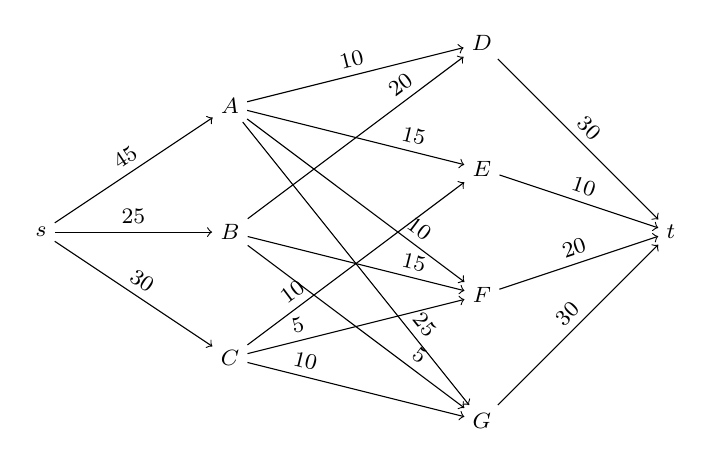
\begin{tikzpicture}[scale=.8] \footnotesize
        \node (f1) at (0, -1) {$A$};
        \node (f2) at (0, -3) {$B$};
        \node (f3) at (0, -5) {$C$};

        \node (p1) at (4, 0) {$D$};
        \node (p2) at (4, -2) {$E$};
        \node (p3) at (4, -4) {$F$};
        \node (p4) at (4, -6) {$G$};

        \node (s) at (-3, -3) {$s$};
        \node (t) at (7, -3) {$t$};

        \begin{scope}[every path/.style={->}]
        \draw (f1) -- (p1) node[midway, above,sloped] {10};
        \draw (f1) -- (p2) node[near end, above,sloped] {15};
        \draw (f1) -- (p3) node[near end, above,sloped] {10};
        \draw (f1) -- (p4) node[near end, above,sloped] {25};
        \draw (f2) -- (p1) node[near end, above,sloped] {20};
        \draw (f2) -- (p4) node[near end, above,sloped] {5};
        \draw (f2) -- (p3) node[near end, above,sloped] {15};
        \draw (f3) -- (p2) node[near start, above,sloped] {10};
        \draw (f3) -- (p3) node[near start, above,sloped] {5};
        \draw (f3) -- (p4) node[near start, above,sloped] {10};

        \draw (s) -- (f1) node[midway, above,sloped] {45};
        \draw (s) -- (f2) node[midway, above,sloped] {25};
        \draw (s) -- (f3) node[midway, above,sloped] {30};
        \draw (p1) -- (t) node[midway, above,sloped] {30};
        \draw (p2) -- (t) node[midway, above,sloped] {10};
        \draw (p3) -- (t) node[midway, above,sloped] {20};
        \draw (p4) -- (t) node[midway, above,sloped] {30};
        \end{scope}

        \end{tikzpicture}
    \end{center}
    \end{exampleblock}
\end{frame}

\begin{frame}{Modélisation de problèmes par un graphe de flot}
    \begin{exampleblock}{Répartition de ressources}
        Pour les problèmes de répartition de ressources, on peut dégager une structure générale :
        \begin{itemize}
            \item Une composante bipartie au centre dont les arêtes modélisent les contraintes de répartition (e.g le débit max d'un tuyau entre un puits et une ville)
            \item Des arêtes entre $s$ et les sources, modélisant les quantités de ressources allouables
            \item Des arêtes entre les destinations et $t$, modélisant les quantités cibles
        \end{itemize}
    \end{exampleblock}
\end{frame}

\begin{frame}{Méthode générale de résolution d'un problème}
    Pour résoudre un problème se modélisant par un graphe de flot (souvent de répartition/affectation de ressources), on suit les étapes suivantes :
    \begin{itemize}
        \item Modéliser le problème par un graphe de flot
        \item Faire tourner l'algorithme de Ford-Fulkerson pour trouver le flot maximal
        \item Extraire la solution du problème du graphe de flots rempli
    \end{itemize}
\end{frame}

% Points importants pour l'examen
\begin{frame}{Conclusion de la section 6}
    Choses à savoir faire pour l'examen :
    \begin{itemize}
        \item Modéliser un problème par un graphe de flot
        \item Faire tourner Ford-Fulkerson à la main sur un exemple pour trouver la solution d'un problème
        \item Connaître et pouvoir raisonner sur les propriétés du flot
    \end{itemize}
    \medskip

    Comment s'entraîner :
    \begin{itemize}
        \item Refaire le TD 6 (exercices 1 et 2)
    \end{itemize}
\end{frame}
